\chapter{Implementation}
%Eigenschaften des Algorithmus, Komplexität, Wie gehen Sie vor?, Beschreiben Sie was wann passiert

After Chapter 4 "System Architecture" has shown an overview of the main components of
the software solution and explained the interaction between them, this chapter explains implementation
details for all major components of the system architecture, including several
collector implementations, as well as the "CollectorClient" and "CollectorManager" component.

The system architecture of the collector platform consists two software components to
be implemented, and the Elasticsearch database, Apache Kafka message broker and the Logstash
indexer to be configured to fulfil the requirements discussed in Chapter 3 and to realize the proposed system architecture in Chapter 4.

The main component, the CollectorClient must provide a REST interface for starting/stopping the collection process
on source systems. Furthermore, it must be possible to fetch metadata about each client. The CollectorManager,
the second software component uses this interface for providing a basic web based UI that lists registered
CollectorClients, shows detailed client information and allows the scheduling the collection process separately
for each client. It follows that two web applications are required, the client application must also be able to
send data to a Apache Kafka, hence the usage of the Procucer API of Kafka must be supported.

The choice for implementing the web applications fell on Spring Boot in the current version 1.4.0. Taken from
the reference documentation \cite{SpringB16}, "Spring Boot makes it easy to create stand-alone, production-grade
Spring based Applications that you can "just run". We take an opinionated view of the Spring platform and
third-party libraries so you can get started with minimum fuss". Features of Spring Boot include the ability to create
standalone web applications conaining an embedded servlet container, what makes the deployment of war files obsolete
and multiple integrations for different applications platforms including Apache Kafka in the subproject spring-kafka.

The following code shows a full example of an web application that provides a simple
HTTP endpoint returning "Hello World". It creates an executable jar file containing
an embedded Apache Tomcat servlet container and can be started from the command line, what means that there is no
dedicated Tomcat instance required to deploy a war file to:

\begin{lstlisting}[caption={Spring Boot "Hello World"}, captionpos=b, label={lst:spring-boot-hello-world}]
@Controller
@EnableAutoConfiguration
public class SampleController {

    @RequestMapping("/")
    @ResponseBody
    String home() {
        return "Hello World!";
    }

    public static void main(String[] args) throws Exception {
        SpringApplication.run(SampleController.class, args);
    }
}
\end{lstlisting}

The Spring framework provides usefull default configurations, thereby making it possible to create a simple Rest service
with just a few annotations. The result is a completely self-contained executable jar, created with the Maven
Buildmanagement tool. Executable jars (sometimes called “fat jars”) are archives containing the compiled classes along with
all of the jar dependencies that the code needs to run. This produces the disadvantage that the memory requirement of the
resulting executable increases. But this was ignored while making the decision for the framework because the presence of
sufficient memory space on Apache Flink and Apache Kafka sources systems had been assumed.

For the implementation of the software components, Java in its version 8 had been chosen. In this current version,
it supports more functional elements in form of lambda expressions, the processing of collections as Streams as well
as an Optional type for handling optional values respectively null values, all features which were used often in the
implementation of the CollectorClient and CollectorManager. Java is the main programming language of Spring Boot, but also
supports Groovy and Scala which did not come into consideration due to the authors lack of experience in these programming
languages.

The software-solution uses Maven as Build- and Dependencymanagement tool, and is divided into the main modules:

\begin{itemize}
	\item collectors
	\item collector-client
	\item collector-manager
	\item collector-data-processor
\end{itemize}

The following sections explains the content and and discusses implementation details for each of these modules separately.

\section{Collectors}

The collector module contains the implementations for the required collectors based on Table 3.4 in
Section 3.1 "Data Quality". It also defines a "collector-commons" module containing basic artifarcts
of the collector domain, common classes and interfaces, that are used and required by the individual
collector implementations

\subsection{Base Domain}

The next class diagramm shows the basic structure, that is equal to all collector implementations on the example
of "JvmCollector":
\begin{figure}[H]
	\centering
	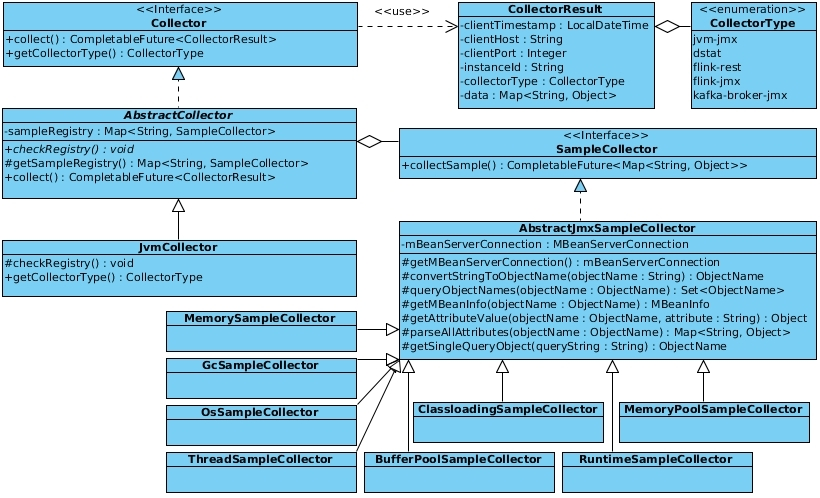
\includegraphics[width=1.0\textwidth]{../uml/class-jvm-collector.jpg}
	\caption{Class diagram 'JvmCollector'}
	\label{class-diagram-jvm-collector}
\end{figure}

This overview describes the collector domain, that is equal to all implementations and consists of following parts:
\begin{enumerate}
    \item \textbf{CollectorType:}
    Enumeration, meta information, that distinguishes collectors implementations
    \item \textbf{CollectorResult:} Data container, the result of a single invocation of the collect() method from
    the Collector interface. Describes a data event, an immutable fact" at a given time, containing the host and port
    the client is running on, the type of collector and the requested data.
    \item \textbf{Collector:} The main interface for implementations, defines the protocol for data collection.
    \item \textbf{AbstractCollector:} Abstract class, provides the implementation of the main collect() method.
    \item \textbf{SampleCollector:} An interface for all classes that collect samples defined by the group the data
    belongs to.
\end{enumerate}

On the example of "JvmCollector", the following section explains the basic design principles that is common
to the main collector domain more in detail wheras only relevant implementation details will be discussed in
subsequent implementations, because the process of collecting data is similar in all.

\subsection{JvmCollector}

The implementation of the Collector interface for fetching "default" JVM data according to Table 3.2 in
Section 3.1.2 "Application Data". This basic set of different management interfaces build the foundation
for the implementation for collecting JVM related data like memory, garbage collector or thread information.

The keep the main implementation as small as possible and following the "Separation Of Concerns" pattern,
the data was divided into different "sample groups", which resulted in one implementation each for collecting
memory, garbage collector or thread data.

A these SampleCollector implementations provide a collectSample() method, that fetches data from a different data group, here
on the example of the class "MemorySampleCollector".

\begin{lstlisting}[caption={MemorySampleCollector collectSample()}, captionpos=b, label={lst:memory-sample-collect}]
private static final String OBJECT_NAME = "java.lang:type=Memory";

@Override
public CompletableFuture<Map<String, Object>> collectSample() {
    return CompletableFuture.supplyAsync(() -> {
        final Map<String, Object> memoryResultMap = Maps.newLinkedHashMap();
        memoryResultMap.put(SAMPLE_KEY, parseMemory(getMemoryMXBean(OBJECT_NAME)));
        return memoryResultMap;
    });
}

private Map<String, Object> parseMemory(final MemoryMXBean proxy) {
    final Map<String, Object> memoryDataMap = Maps.newLinkedHashMap();
    memoryDataMap.put(MEMORY_OPFC_KEY, proxy.getObjectPendingFinalizationCount());
    return memoryDataMap;
}

private MemoryMXBean getMemoryMXBean(final String objectName) {
    try {
        return ManagementFactory.newPlatformMXBeanProxy(mBeanServerConnection(), objectName, MemoryMXBean.class);
    } catch (IOException ex) {
        throw ex;
    }
}
\end{lstlisting}

As one of the non functional requirements in Chapter 3, the client implementation may not cause a negative impact
on source systems regarding system resources like cpu or disk usage. To make the code as "non-blocking" as possible,
the implementation is based on the usage of CompletableFutures. It models an asynchronous computation and provides
a reference to its results that will be available when the computation itself is completed. These computations like the JMX
access in the example above, are potentially time-consuming \cite{TODO}. The CompletableFuture allows the caller thread to return immediately
to perform other operations instead of waiting for the result of the computation of JMX memory data, by delegating to a
separate thread performing the operations defined in the CompletableFuture.

The code in line 1-8 wraps the computation of JMX memory data, which contains the data access via the MBeanServerConnection,
introduced in Chapter 2 "Basic Concepts", and the preparation of result data in a separate thread performing the operations defined
in the futures method body.

The implementations for the other SampleCollectors are almost the same, it only differs in the JMX management bean the data will
be queried from.

Every collector implementation is based on an internal registry of SampleCollectors, every implementation must provide its
own registry required for the main collector process, that delegates to its registered SampleCollectors,
aggregates their results and creates the overall result of the collector. To split the collection into individual sample groups has
the advantage, that it makes the implementation very flexible regarding the data to collect. To add further data sources, it
will be enough to provide an implementation of the SampleCollector interface and to add an entry to the registry.

\begin{lstlisting}[caption={Sample registry for "JvmCollector"}, captionpos=b, label={lst:jvmsampleregistry}]
private static Map<String, SampleCollector> jvmSampleRegistry(final MBeanServerConnection mBeanServerConnection) {
    final Map<String, SampleCollector> registry = Maps.newHashMap();
    registry.put(MemorySampleCollector.SAMPLE_KEY, new MemorySampleCollector(mBeanServerConnection));
    registry.put(ThreadSampleCollector.SAMPLE_KEY, new ThreadSampleCollector(mBeanServerConnection));
    ...
    return registry;
}

@Override
public CollectorType getCollectorType() {
    return CollectorType.JVM_JMX;
}

@Override
protected void checkRegistry() {
    if (getSampleRegistry().isEmpty()) {
        throw new JmxCollectorException();
    }
}
\end{lstlisting}

The rest of the JvmCollector code consists of required method implementations of abstract methods defined in the class
AbstractCollector. Due to the fact that a concrete collector implementation only require that less code









\subsection{AbstractCollector}

\subsection{FlinkRestCollector}

%

%
%TODO: Collector results aggregated of sample collector results, extensibility for further sample sources
%
%\begin{lstlisting}[caption={The "collect"-algorithm in "AbstractCollector"}, captionpos=b, label={lst:abstractcollectorcollect}]
%@Override
%public CompletableFuture<CollectorResult> collect() {
%    LOG.debug("Entering AbstractCollector collect()");
%    final CompletableFuture<CollectorResult> collectorResultCF = CompletableFuture.supplyAsync(() -> {
%    checkRegistry();
%    final List<CompletableFuture<Map<String, Object>>> sampleResultCPList =
%        getSampleRegistry().values().stream()
%                    .map(SampleCollector::collectSample)
%                    .collect(Collectors.toList());
%
%    return CompletableFuture.allOf(sampleResultCPList.toArray(
%        new CompletableFuture[sampleResultCPList.size()]))
%            .thenApply(aVoid ->
%                sampleResultCPList.stream().map(CompletableFuture::join)
%                    .collect(Collectors.toList()))
%            .thenApply(sampleResults -> {
%                final Map<String, Object> dataMap = Maps.newLinkedHashMap();
%                sampleResults.forEach(dataMap::putAll);
%                final CollectorResult collectorResult =
%                    new CollectorResult(getCollectorType().name().toLowerCase(), dataMap);
%                LOG.debug("Finished AbstractCollector collect()");
%                return collectorResult;
%            }).join();
%        });
%        LOG.debug("Immediately return from AbstractCollector collect()");
%        return collectorResultCF;
%}
%\end{lstlisting}
%
\subsection{CollectorType}
%
%TODO: Distinguishes collectors, meta information not neccessarily required
%
%\begin{lstlisting}[caption={Collector types}, captionpos=b, label={lst:collectortypesimpl}]
%public enum CollectorType {
%    JVM_JMX,
%    DSTAT,
%    FLINK_REST,
%    FLINK_JMX,
%    KAFKA_BROKER_JMX
%}
%\end{lstlisting}
%
%\begin{lstlisting}[caption={CollectorResult}, captionpos=b, label={lst:collectortypesimpl}]
%public class CollectorResult {
%    @JsonProperty("client-timestamp")
%    private final LocalDateTime clientTimestamp;
%
%    @JsonProperty("client-host")
%    private final String clientHost;
%
%    @JsonProperty("client-port")
%    private final Integer clientPort;
%
%    @JsonProperty("instance-id")
%    private final String instanceId;
%
%    @JsonProperty("collector-type")
%    private final String collectorType;
%
%    private final Map<String, Object> data;
%}
%\end{lstlisting}

%
\subsection{DStatCollector}
%
%Dstat parameters, see Table 3.1 in Chapter "Basic Concepts"
%
%\begin{lstlisting}[caption={Dstat program parameters in "DstatCollector"}, captionpos=b, label={lst:dstatparameters}]
%private static final String[] DSTAT_COMMAND = {"dstat", "-t",
%    "--cpu", "--top-cpu-adv", "--top-cputime", "--top-cputime-avg",
%    "--disk", "--disk-tps", "--disk-util",
%    "--net", "--socket", "--tcp", "--udp",
%    "--io", "--top-io-adv", "--lock", "--fs",
%    "--mem", "--top-mem", "--page", "--swap", "--vm",
%    "--sys", "--load", "--ipc", "--unix",
%    "--proc", "--proc-count", "--top-latency", "--top-latency-avg",
%    "--full",
%    "--float", "1", "0"};
%\end{lstlisting}

%Dstat process with the given parameters results in string containing three lines, where only the third line ist required to
%to gather data of.

%All collector implementations use a sample registry to achieve more flexibility in what data to collect:
%\begin{lstlisting}[caption={Sample registry in "DstatCollector"}, captionpos=b, label={lst:dstatsampleregistry}]
%private static Map<String, AbstractDstatSampleCollector> defaultSampleRegistry() {
%    final Map<String, AbstractDstatSampleCollector> registry = Maps.newHashMap();
%    registry.put(CpuSampleCollector.SAMPLE_KEY, new CpuSampleCollector());
%    registry.put(DiskSampleCollector.SAMPLE_KEY, new DiskSampleCollector());
%    registry.put(IoSampleCollector.SAMPLE_KEY, new IoSampleCollector());
%    registry.put(MemorySampleCollector.SAMPLE_KEY, new MemorySampleCollector());
%    registry.put(NetSampleCollector.SAMPLE_KEY, new NetSampleCollector());
%    registry.put(ProcessSampleCollector.SAMPLE_KEY, new ProcessSampleCollector());
%    registry.put(SystemSampleCollector.SAMPLE_KEY, new SystemSampleCollector());
%    return registry;
%}
%\end{lstlisting}
%
%Java ProcessBuilder to create Dstat process and read output using an InputStreamReader provided by the Process object.
%\begin{lstlisting}[caption={ProcessBuilder in "DstatCollector"}, captionpos=b, label={lst:dstatprocessbuilder}]
%final ProcessBuilder processBuilder = new ProcessBuilder(DSTAT_COMMAND);
%processBuilder.redirectErrorStream(true);
%final Process process = processBuilder.start();
%try (BufferedReader processOutputReader =
%    new BufferedReader(new InputStreamReader(process.getInputStream()))) {
%        final String dstatResult = processOutputReader.lines()
%            .map(String::toString)
%            .collect(Collectors.joining(System.lineSeparator()));
%        final int exitCode = process.waitFor();
%}
%\end{lstlisting}
%
%The result will be splitted by System.lineSeparator in AbstractDstatSampleCollector. Implements Function<String, Map<String, Object>>,
%a functional interface that takes on input and creates a result on apply.
%\begin{lstlisting}[caption={Split Dstat input in "AbstractDstatSampleCollector"}, captionpos=b, label={lst:dstatsplitdat}]
%@Override
%public Map<String, Object> apply(final String dstatResult) {
%    final String[] lines = dstatResult.split(System.lineSeparator());
%        if (lines.length != 3) {
%            throw new DStatCollectorException();
%        }
%    return createResultMap(applyData(lines));
%}
%\end{lstlisting}
%
%DstatCollector iterates through sample registry and invokes "collect" for all registred sample collector implementations.
%Usage of futures for non-blocking code, block as less as possible to increase performance on source systems.
%\begin{lstlisting}[caption={Iterate sample registry in "DstatCollector"}, captionpos=b, label={lst:dstatiterate}]
%final List<CompletableFuture<Map<String, Object>>> dStatDataFuturesList =
%    sampleRegistry.values().stream()
%        .map(collector ->
%            CompletableFuture.supplyAsync(() ->
%                collector.apply(dstatResult))).collect(Collectors.toList());
%\end{lstlisting}
%
%All Dstat sample collectors are based on regular expressions, the third line of the result is splitted, and the data of interest
%extracted:
%\begin{lstlisting}[caption={Extract sample date in  "CpuSampleCollector"}, captionpos=b, label={lst:cpusamplecollector}]
%CPU_USAGE_PATTERN = Pattern.compile("" +
%    "(\\d+(\\.\\d+)?)(\\s*)" +
%    "(\\d+(\\.\\d+)?)(\\s*)" +
%    "(\\d+(\\.\\d+)?)(\\s*)" +
%    "(\\d+(\\.\\d+)?)(\\s*)" +
%    "(\\d+(\\.\\d+)?)(\\s*)" +
%    "(\\d+(\\.\\d+)?)");
%
%private static Map<String, Object> parseCpuUsage(final String rawData, final String cpuName) {
%    return Optional.ofNullable(rawData).map(raw -> {
%        final Matcher matcher = CPU_USAGE_PATTERN.matcher(raw.trim());
%        final Map<String, Object> cpuUsageMap = Maps.newLinkedHashMap();
%        if (!matcher.matches()) {
%            LOG.warn("Unable to parse 'CpuUsage'");
%        } else {
%            try {
%                cpuUsageMap.put(CPU_NAME_KEY, cpuName);
%                cpuUsageMap.put(CPU_USAGE_USER_KEY, Float.valueOf(matcher.group(1)));
%                cpuUsageMap.put(CPU_USAGE_SYSTEM_KEY, Float.valueOf(matcher.group(4)));
%                ...
%            } catch (NumberFormatException ex) {
%                LOG.warn("Unable to parse 'CpuUsage'");
%            }
%        }
%        return cpuUsageMap;
%    }).orElse(Maps.newHashMap());
%}
%\end{lstlisting}
%
%At the end of Dstat collection, the futures of the different sample collectors will be aggregated
%to one CollectorResult future, that will be returned to the caller of the collect() method of DstatCollector.
%\begin{lstlisting}[caption={Aggregation of sample results in "DstatCollector"}, captionpos=b, label={lst:dstatsampleaggregation}]
%dStatDataFuturesList
%    .stream()
%        .map(CompletableFuture::join)
%            .collect(Collectors.toList()))
%                .thenApply(dstatSamples -> {
%                    final Map<String, Object> data = Maps.newLinkedHashMap();
%                    dstatSamples.forEach(data::putAll);
%                    final CollectorResult dstatCollectorResult = new CollectorResult(CollectorType.DSTAT.name().toLowerCase(), data);
%                    LOG.debug("Finished {} collecting", CollectorType.DSTAT);
%                    return dstatCollectorResult;
%                    }).join();
%\end{lstlisting}



\subsection{KafkaBrokerJmxCollector}



\section{CollectorClient}

\subsection{CollectorWorker}

\subsection{KafkaOutboundWriter}

\subsection{ScheduleController}

\subsection{ClientMetadataController}

\section{CollectorManager}

\subsection{CollectorClientInstanceService}

\subsection{MetadataRestClient}

\subsection{IndexController}

\section{Summary}

%According to the functional requirements
%discussed in Chapter 3 "Requirements and Specification", any other programming language could had been used, as long
%it is possible to provide and consume a RESTfull API and integration for the Producer and Consumer API of Apache
%Kafka is available.

Maybe Spring alternatives, Lagom, VertX, Play?

Maybe collector as agent, Instrumentation instead of separate service

Alternatives REST, maybe (Web-)Sockets

Possible secururity risk because remote JMX, firewalls